\documentclass[12pt]{article}
\usepackage{amsmath}
\usepackage{amssymb}
\usepackage[letterpaper,top=0.75in,bottom=1in,left=0.75in,right=0.75in,centering]{geometry}
%\usepackage{fancyhdr}
\usepackage{enumerate}
%\usepackage{lastpage}
\usepackage{multicol}
\usepackage{graphicx}

\usepackage{tikz}
\usetikzlibrary{calc, positioning, decorations.pathmorphing}

%\reversemarginpar

%\pagestyle{fancy}
%\cfoot{}
%\lhead{Math 1560}\chead{Test \# 1}\rhead{May 18th, 2017}
%\rfoot{Total: 10 points}
%\chead{{\bf Name:}}
\newcommand{\points}[1]{\marginpar{\hspace{24pt}[#1]}}
\newcommand{\skipline}{\vspace{12pt}}
%\renewcommand{\headrulewidth}{0in}
\headheight 30pt

\newcommand{\di}{\displaystyle}
\newcommand{\abs}[1]{\lvert #1\rvert}
\newcommand{\len}[1]{\lVert #1\rVert}
\renewcommand{\i}{\mathbf{i}}
\renewcommand{\j}{\mathbf{j}}
\renewcommand{\k}{\mathbf{k}}
\newcommand{\R}{\mathbb{R}}
\newcommand{\aaa}{\mathbf{a}}
\newcommand{\bbb}{\mathbf{b}}
\newcommand{\ccc}{\mathbf{c}}
\newcommand{\dotp}{\boldsymbol{\cdot}}
\newcommand{\bbm}{\begin{bmatrix}}
\newcommand{\ebm}{\end{bmatrix}}                   
\DeclareMathOperator{\dom}{dom}

\begin{document}


\begin{center}
Math 1565 Tutorial \#3 Solutions
\end{center}
\begin{enumerate}
 \item  For this problem you may use the fact (proven in class) that $g(x)=\abs{x}$ is continuous on $\R$.
 \begin{enumerate}
 \item Prove that if $f$ is continuous, then $\abs{f}$ is continuous.
 
 \medskip
 
\textbf{Solution:} With $g(x)=\abs{x}$, the absolute value of any function $f$ is given by the composition $\abs{f} = g\circ f$; that is, for each $x\in\dom(f)$, $\abs{f(x)} = g(f(x))$.

Since the composition of continuous functions is continuous, the result follows.

\medskip
 
 \item Give a counterexample showing that the converse to part (a) is false. That is, find a function $f$ such that $\abs{f}$ is continuous everywhere, but $f$ is not.

\medskip

\textbf{Solution:} There are plenty of examples that work; a particularly simple one is
\[
f(x) = \begin{cases}1, & \text{ if } x\geq 0\\-1, & \text{ if } x<0\end{cases}.
\]
It's clear that $f$ has a jump discontinuity at $x=0$, but since $\abs{f(x)} = 1$ for all $x\in \R$, $\abs{f}$ is the constant function 1, which is continuous.
 \end{enumerate}
 
\bigskip
 
 \item On what intervals is $x^2<x^4$? On what intervals is $x^4<x^2$? If the graph of $f(x)$ always lies between the graphs $y=x^2$ and $y=x^4$, for what real numbers $a$ can you determine the value of $\lim_{x\to a}f(x)$ using the Squeeze Theorem? Find these values.

\medskip

\textbf{Solution:} We see that
\[
x^2<x^4 \Leftrightarrow x^4-x^2>0 \Leftrightarrow x^2(x-1)(x+1)>0.
\]
The sign diagram for this inequality is given by
\begin{center}
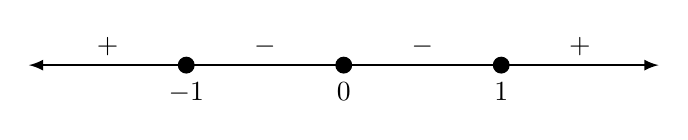
\begin{tikzpicture}[>=latex]
  \draw [thick, <->] (-4,0) -- (4,0);
  \draw [fill] (-2,0) circle [radius =.1];
  \draw [fill] (0,0) circle [radius =.1];
  \draw [fill] (2,0) circle [radius =.1];
  \node at (-3,0) [above] {$+$};
  \node at (-1,0) [above] {$-$};
  \node at (1,0) [above] {$-$};
  \node at (3,0) [above] {$+$};
  \node at (-2,-0.1) [below] {$-1$};
  \node at (0,-0.1) [below] {$0$};
  \node at (2,-0.1) [below] {$1$};
  \end{tikzpicture}
\end{center}
From the sign diagram, we can conclude that $x^2<x^4$ for $x\in (-\infty, -1)\cup(1,\infty)$, while $x^4<x^2$ for $x\in (-1,0)\cup (0,1)$.

The Squeeze Theorem can be applied at the three points where the graphs $y=x^2$ and $y=x^4$ intersect;* namely $x=-1,0,1$.

If the graph of $f(x)$ lies between these two graphs, we would have
\[
\lim_{x\to -1}f(x) = 1, \lim_{x\to 0}f(x) = 0, \text{ and } \lim_{x\to 1}f(x) = 1.
\]

*Note that $x=0$ is the only point where the Squeeze Theorem can be applied without a bit of extra caution, since we have $x^4<x^2$ on both sides of $x=0$, and thus it is possible for the inequality $x^4\leq f(x)\leq x^2$ to hold on an interval containing zero.

At $x=\pm 1$, we need to be more careful, since the inequality changes depending on which side of these points we're on. The Squeeze Theorem can still be applied, but technically, one must consider left and right hand limits separately, since a different inequality is needed on either side of the point.


 
 \item Consider the function $f(x)=x^3+2x^2-1$.
 \begin{enumerate}
 \item Prove that $f$ has a root ($x$-intercept) in $[0,1]$.
 
 \medskip
 
\textbf{Solution:} We note that $f$ is continuous on $[0,1]$, since it is a polynomial function, and $f(0)=-1<0$, while $f(1) = 2>0$. Thus, by the Intermediate Value Theorem, there must exist some $c\in (0,1)$ such that $f(c)=0$.

\bigskip
 
 \item Determine an interval of length $1/16$ containing the root from part (a).
 
 \medskip
 
\textbf{Solution:} We use the Bisection Method. The midpoint of $[0,1]$ is $1/2$. We find
\[
f(1/2) = \frac{1}{8}+2\cdot\frac{1}{4}-1 = -\frac{3}{8}<0.
\]
Since $f(1/2)<0$ but $f(1)>0$, we conclude that our root lies in the interval $(1/2,1)$. The midpoint of this interval is $3/4$. We find
\[
f(3/4) = \frac{27}{64}+2\cdot \frac{9}{16}-1 = \frac{35}{64}>0.
\]
Since $f(1/2)<0$ but $f(3/4)>0$, we conclude that our root lies in the interval $(1/2,3/4)$. The midpoint of this interval is $5/8$. We find
\[
f(5/8) = \frac{125}{512}+2\cdot \frac{25}{64}-1 = \frac{13}{512}>0.
\]
Since $f(1/2)<0$ but $f(5/8)>0$, we conclude that our root lies in the interval $(1/2,5/8)$. The midpoint of this interval is $9/16$, and we find
\[
f(9/16) = \frac{729}{4096}+2\cdot \frac{81}{256}-1 = -\frac{775}{4096}<0.
\]
Since $f(9/16)<0$ but $f(5/8)>0$, we conclude that the root must lie in the interval $(9/16, 5/8)$, which has length $1/16$, as required.
 \end{enumerate}


\end{enumerate}
\end{document}